\documentclass[oneside,14pt]{extarticle}
\usepackage[utf8]{inputenc}
\usepackage[english,ukrainian]{babel}
\usepackage{amssymb,amsfonts,amsmath,amsthm,mathtext,textcomp}

\usepackage[includehead, headsep=0pt, footskip=0pt, top=2cm, bottom=2cm, left=2cm, right=1cm]{geometry}
\usepackage{indentfirst}
\usepackage[onehalfspacing]{setspace}
\usepackage[headings]{fancyhdr}
\usepackage{etoolbox}
\usepackage{flafter}
\usepackage{listings}
\usepackage{graphicx}
\usepackage{float}
\usepackage[labelsep=period]{caption}

\usepackage{array}
\fancyhf{}
\renewcommand{\headrulewidth}{0pt}
\pagestyle{fancy}
\fancyfoot[R]{\thepage}
\lstset{breaklines=true,}
\graphicspath{ {./pictures} }

\lstset{
	language=c,
	tabsize=4,
	keepspaces,
	showstringspaces=false,
}
\graphicspath{ {./pictures} }
\setlength{\parindent}{4em}

\newcommand\subject{Програмування в Інтернет}
\newcommand\lecturer{асистент кафедри ПЗ \\ Степанов Д. С.}
\newcommand\teacher{старший викладач кафедри ПЗ \\ Грицай О. Д.}
\newcommand\mygroup{ПЗ-22}
\newcommand\lab{1}
\newcommand\theme{Структура DOM та методи доступу до вузлів дерева}
\newcommand\purpose{Ознайомитись з ієрархічною структурою об’єктів JavaScript та об’єктами
	документа і браузера}

\begin{document}
\begin{normalsize}
	\begin{titlepage}
		\thispagestyle{empty}
		\begin{center}
			\textbf{МІНІСТЕРСТВО ОСВІТИ І НАУКИ УКРАЇНИ\\
				НАЦІОНАЛЬНИЙ УНІВЕРСИТЕТ "ЛЬВІВСЬКА ПОЛІТЕХНІКА"}
		\end{center}
		\begin{flushright}
			\textbf{ІКНІ}\\
			Кафедра \textbf{ПЗ}
		\end{flushright}
		\vspace{70pt}
		\begin{center}
			\textbf{ЗВІТ}\\
			\vspace{10pt}
			до лабораторної роботи № \lab\\
			\textbf{на тему}: “\textit{\theme}”\\
			\textbf{з дисципліни}: “\subject”
		\end{center}
		\vspace{50pt}
		\begin{flushright}
			
			\textbf{Лектор}:\\
			\lecturer\\
			\vspace{10pt}
			\textbf{Виконав}:\\
			
			студент групи \mygroup\\
			Коваленко Д.М.\\
			\vspace{10pt}
			\textbf{Прийняв}:\\
			
			\teacher\\
			
			\vspace{28pt}
			«\rule{1cm}{0.15mm}» \rule{1.5cm}{0.15mm} 2023 р.\\
			$\sum$ = \rule{1cm}{0.15mm}……………\\
			
		\end{flushright}
		\vspace{\fill}
		\begin{center}
			\textbf{Львів — 2023}
		\end{center}
	\end{titlepage}
		
	\begin{description}
		\item[Тема.] \theme.
		\item[Мета.] \purpose.
	\end{description}

	\section*{Завдання}
	\begin{figure}[H]
		\centering
		
\includegraphics[scale=0.7]{v}
	\end{figure}

	\section*{Теоретичні відомості}
	Web-сторінка може мати вигляд дерева, вузли якого є об’єктами, до властивостей
	яких доступаються операторами мови програмування Javascript.
	Модель DOM (Document Object Model, об’єктна модель документа) містить низку
	стандартних глобальних об’єктів. Зокрема, це window, navigator, document,
	screen, history, location.
	
	Події та обробники подій є дуже важливою частиною у програмування на JavaScript.
	Події (Events), головним чином, ініціюються тими або іншими діями користувача. Події –
	це дії, які відбуваються, внаслідок того, що робить користувач. Наприклад, якщо
	користувач клацає по деякій кнопці, відбувається подія Click. Якщо миша перетинає
	яке-небудь посилання - відбувається подія MouseOver. Існує певний набір подій, які
	розпізнає той чи інший броузер.
	
	Ви можете поміщати будь-які твердження JavaScript усередині кавичок onClick. Ці
	твердження будуть виконані, коли користувач натискатиме на кнопку. Якщо Ви хочете
	включити більш ніж одне твердження, то окремі твердження записуються через крапку з
	комою (;).
	Взагалі, це – непогана ідея визначати функцію для обробників подій тому що: це робить ваш код мобільним, оскільки ви можете використовувати ту ж саму
	функцію в багатьох різних місцях це робить ваші твердження більш легкими для читання.

	\section*{Хід виконання}
	Посилання на код:\\ $https://gitlab.com/geekylthyosaur/web/-/tree/main/lab1$
	
	Створення header'у сторінки:
	
	html:
	\begin{lstlisting}
<header>
<div class=``logo''>
<a href=``\#''>Logo</a>
</div>


<div class=``user''>
<div id=``notification-header-trigger''>
<div class=``user-notification''>
<i class=``fa fa-bell-o''></i>
<span class=``badge''></span>
</div>
</div>

<div id=``profile-header-trigger''>
<a href=``\#'' class=``user-name''>John Doe</a>
<a href=``\#'' class=``user-img fa fa-user-circle-o''></a>
</div>

<div id=``profile-header'' class=``profile-header''>
<a href=``\#'' class=``profile-button''>Profile</a>
<br>
<a href=``\#'' class=``logout-button''>Log Out</a>
</div>

<div id=``notification-header'' class=``notification-header''>
<span class=``fa fa-user-circle-o''>
<a href=``\#''>Admin</a>
</span>
<div class=``notification-msg''></div>
<span class=``fa fa-user-circle-o''>
<a href=``\#''>Joe Biden</a>
</span>
<div class=``notification-msg''></div>
</div>
</div>
</header>
	\end{lstlisting}

css:

	\begin{lstlisting}
header {
	background-color: #333;
	color: #fff;
	display: flex;
	justify-content: space-between;
	align-items: center;
	padding: 20px;
	margin: -10px;
}

.logo a {
	color: #fff;
}

.user {
	display: flex;
	justify-content: flex-end;
	align-items: center;
}

.user a {
	margin-left: 10px;
	color: #fff;
}

.user-name {
	padding-left: 20px;
}

.user-notification {
	position: relative;
	display: inline-block;
}

.user-notification .badge {
	position: absolute;
	top: -10px;
	right: -10px;
	background-color: red;
	color: white;
	padding: 5px;
	border-radius: 50%;
	animation: blink 1s infinite;
}

@keyframes blink {
	0% {
		opacity: 1;
	}
	50% {
		opacity: 0;
	}
	100% {
		opacity: 1;
	}
}
	\end{lstlisting}

	Створення таблиці:
	
	html:
	\begin{lstlisting}
<div class="content">
<h1>Students</h1>
<button id="add-row" class="add-row btn fa fa-plus-square-o"></button>
<table id="table">
<tr>
<th><input type="checkbox" id="check-all"></th>
<th>Group</th>
<th>Name</th>
<th>Gender</th>
<th>Birthday</th>
<th>Status</th>
<th>Options</th>
</tr>
</table>
</div>
</div>
	\end{lstlisting}

	css:
	\begin{lstlisting}
table, th, td {
	border: 1px solid;
	border-collapse: collapse;
	border-color: gray;
}

table {
	width: 100%;
}

th, td {
	text-align: center;
	padding: 8px;
}

ul {
	list-style: none;
	margin: 0;
	padding: 0;
}

li {
	display: block;
	text-align: left;
}

li {
	display: block;
	text-align: left;
	padding: 10px 0;
}

a {
	text-decoration: none;
	color: #333;
}
	\end{lstlisting}

\begin{figure}[H]
	\centering
	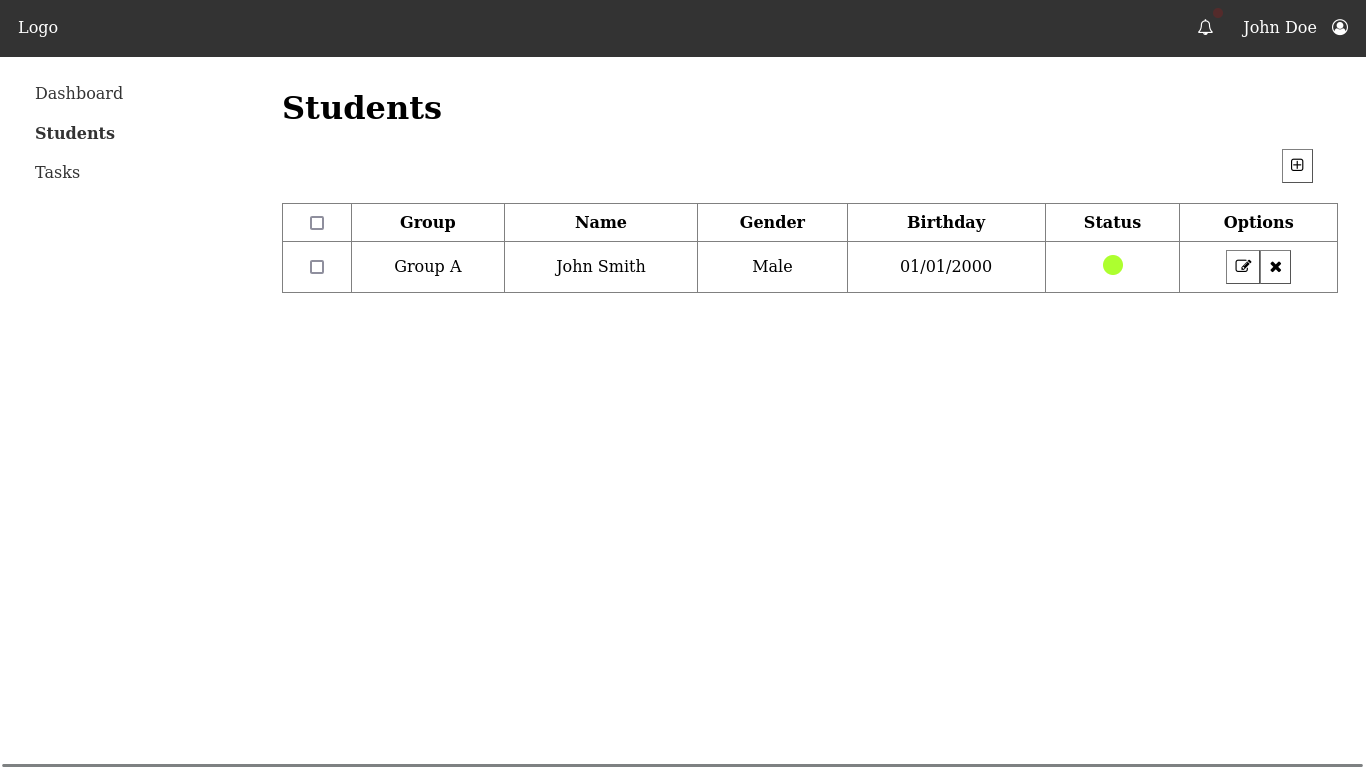
\includegraphics[scale=0.35]{3}
	\caption{Вигляд сторінки}
\end{figure}

	\begin{figure}[H]
		\centering
		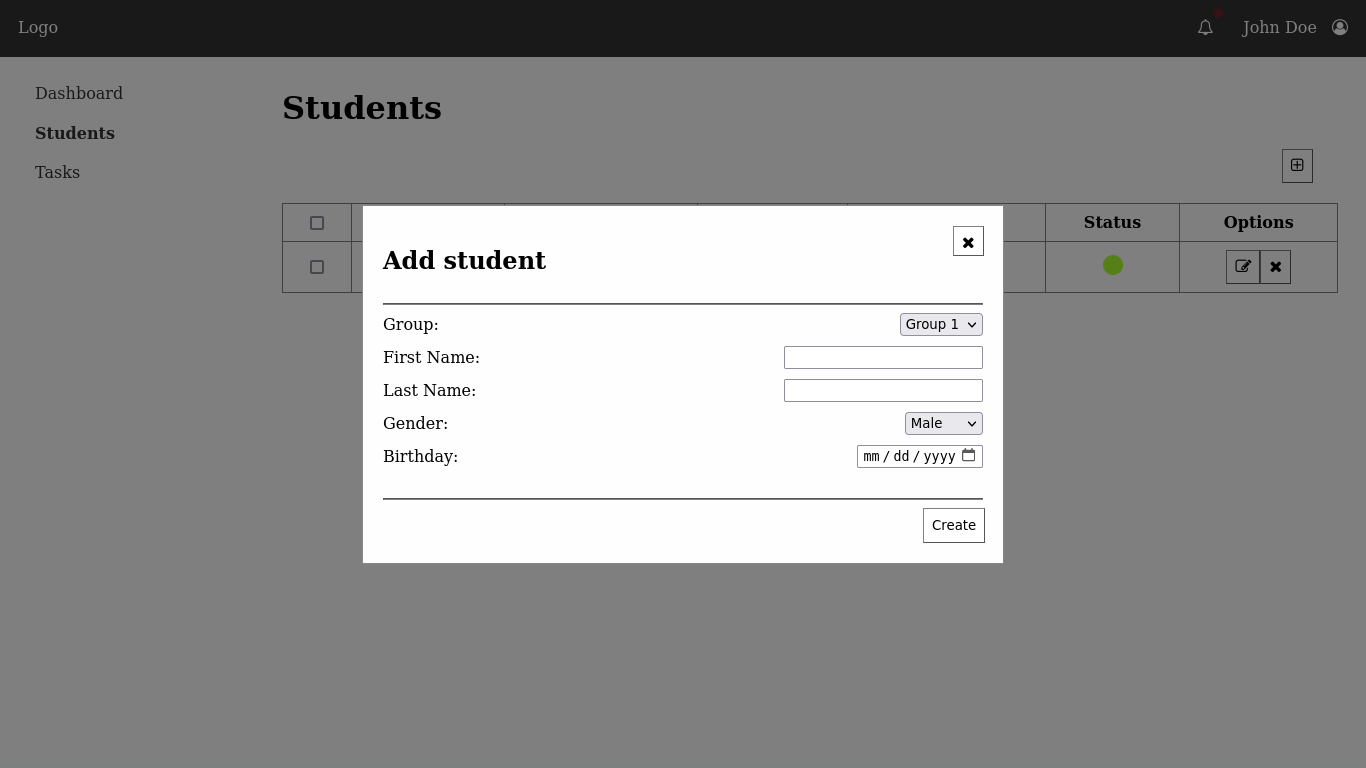
\includegraphics[scale=0.35]{1}
		\caption{Видалення студента з таблиці}
	\end{figure}

	\begin{figure}[H]
		\centering
		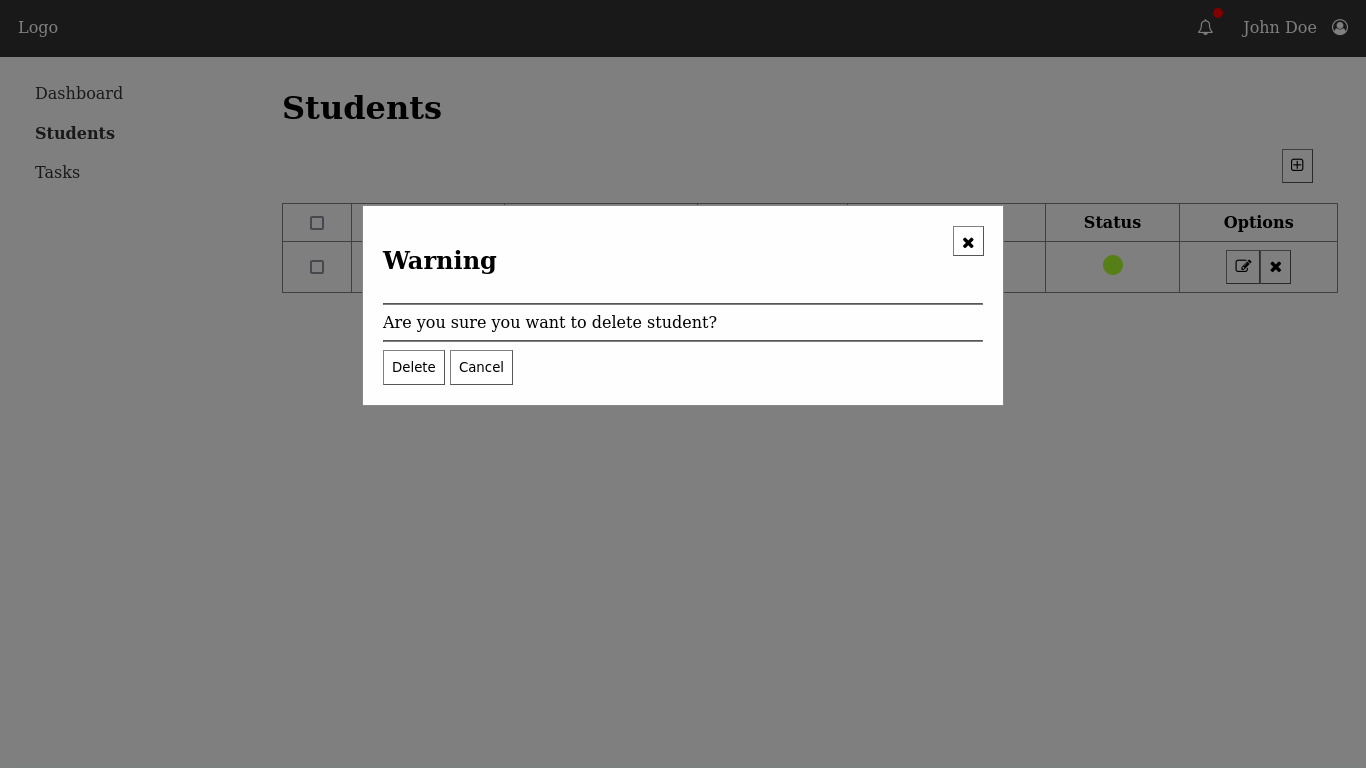
\includegraphics[scale=0.35]{2}
		\caption{Додавання студента до таблиці}
	\end{figure}

	\section*{Висновки}
	Під час виконання лабораторної роботи я ознайомився з ієрархічною структурою об’єктів JavaScript та об’єктами
	документа і браузера. Навчився працювати з анімаціями засобами CSS. З додаванням та видаленням елементів HTML засобими JavaScript.
	    
\end{normalsize}
\end{document}
